\chapter{Processamento de Linguagem Natural}
\label{cap:Processamento}

% Um computador, obviamente, está preparado para entender sua própria linguagem,
% como por exemplo, um compilador interpreta linhas de código fonte para gerar um
% programa executável seguindo exatamente o algoritmo utilizado. Por isso, temos o
% termo Natural no Processamento de Linguagem.

O objetivo da área de Processamento de Linguagem Natural é analisar a linguagem
natural, ou seja, a linguagem utilizada pelo seres humanos seja ela escrita
ou falada \cite{manningschutze1999}. O Processamento de Linguagem Natural é uma
área antiga, sendo anterior a invenção dos computadores modernos. De fato, sua primeira grande aplicação foi
um dicionário desenvolvido no Birkbeck College em Londres no ano de 1948. Por ser
uma área complexa, seus primeiros trabalhos foram notavelmente falhos, o que
causou uma certa hostilidade por parte das agências fomentadoras de pesquisas.

Os primeiros pesquisadores eram muitas vezes bilíngues, como por exemplo,
nativos alemães que imigraram para os Estados Unidos. Acreditava-se que pelo
fato desses terem conhecimento de ambas as linguas, Ingles e Alemão, eles teriam
capacidade de desenvolver programas de computadores que efetuariam a tradução
de modo satisfatório. Uma vez que esses encontraram muitas dificuldades,
ficou claro que o maior problema não era o conhecimento das
línguas, e sim como expressar esse conhecimento na forma de um programa de
computador \cite{history}.

Para que um computador seja capaz de interpretar uma
língua, primariamente, necessitamos compreender como nós efetuamos essa
interpretação.
Por isso, uma parte considerável do Processamento de Linguagem Natural está apoiado na área de Linguística.

\newpage

\section{Linguística}

O objetivo da Linguística é compreender como os seres humanos adquirem, produzem
e entendem as diversas línguas, ou seja, a forma como conversamos, a nossa
escrita e outras mídias de comunicação \cite{manningschutze1999}.

Na linguagem tanto escrita, como na falada, existem regras gramaticais que são
utilizadas para estruturar as expressões. Uma série de dificuldades no Processamento de
Linguagem Natural são ocasionadas pelo fato de que as pessoas constantemente
mudam essas regras para satisfazerem suas necessidades de comunicação
\cite{manningschutze1999}. Uma vez que as regras são constantemente modificadas
pelo locutor, torna-se extremamente difícil a criação de um software ou hardware
que efetue a interpretação de uma língua.


% \subsection{Sintaxe e Semântica}
%
% No seu livro Estruturas Sintáticas, Noam Chomsky cita as seguintes frases
% ``Ideias verdes incolores dormem furiosamente'' e ``Incolores verde ideias dormem
% furiosamente''.
%
% A primeira frase, do ponto de vista sintático é correta, porém, assim como a
% segunda frase, semânticamente não faz sentido.
%
% O fato de que podemos modificar as regras da lingua de duas formas distintas é
% utilizado como evidência para a separação da sintaxe e semântica na língua.
% \cite{jacksonmoulinier2007}

\section{Métodos de Processamento de Linguagem Natural}

O \ac{NLP} tem como objetivo a execução de diferentes tarefas, como por exemplo,
a categorização de documentos, a tradução e a geração de textos a partir de um
banco de dados, etc. Podemos citar duas classes de métodos para a execução deste
tipo de tarefas, que são os métodos simbólicos e os métodos estatísticos.

Nos final dos anos 50 e 60, existiam excelentes métodos estatísticos, que foram
desenvolvidos durante a segunda guerra mundial, para a solução de problemas
Linguísticos \cite{shannon48}.
Porém, no ano de 1957, Chomsky publicou o trabalho intitulado de
\textit{``Syntactic Structures''} onde descreve a
teoria da gramática gerativa, que é uma teoria que considera a
gramática como um conjunto de regras. Essa abordagem através de um conjunto de
regras, ao invés de um modelo estatístico, entra em conflito com os trabalhos
anteriores, criando duas comunidades no campo da Linguística. Como reflexo
dessas duas comunidades, a área de \ac{NLP} que crescia em paralelo, também foi
dividida em duas áreas. A primeira dessas áreas que fazia uso de métodos
baseados em regras (simbólica) e a segunda que fazia o uso de métodos quantitativos (estatística).


Nesta seção será apresentado um exemplo de um método simbólico e de um método
estatístico.
Destaca-se que a descrição realizada nesta seção apresenta como objetivo, apenas
diferenciar ambas as classes de métodos, através de seus requisitos e forma de execução.
Destaca-se ainda que os métodos apresentados nesta seção não são utilizados na
análise de sentimentos, sendo que os métodos específicos para essa
análise serão descritos no Capítulo \ref{cap:Classificadores}.


\subsection{Método Simbólico}
O método simbólico ou racionalista está
baseado no campo da Linguística e faz o uso da manipulação dos símbolos,
significados e das regras de um texto. Um exemplo simples de um método simbólico
é o método de Brill \cite{Brill:1992:SRP:974499.974526} utilizado para a
análise léxica, ou seja, identificar a classe de uma palavra em um texto.
Por exemplo, no método de Brill a frase ``João pintou a casa de branco'', será separada em palavras que
serão classificadas através de um dicionário pré-definido, como:

\begin{table}[htb]
\centering
\begin{tabular}{l|l|l|l|l|l|l}
Palavra         & João        & pintou & a      & casa        & de
& branco
\\
%Correta: & Substantivo & Verbo  & Artigo & Substantivo & Preposição &
% Substantivo \\
Classificação:   & 			   & Verbo  & Artigo & Substantivo & Preposição & Adjetivo
\end{tabular}
\label{my-label}
\end{table}

Observa-se que algumas palavras não foram
identificadas, como ``João'', ou classificadas de forma incorreta, como
``branco". Desta forma, o método de Brill utiliza-se de outras duas regras para
a classificação.
A primeira dessas regras classifica todas as palavras desconhecidas que
iniciam com uma letra em maiúscula como substantivos, por exemplo, a palavra ``João''. Já a
segunda regra, atribui para a palavra desconhecida a mesma classificação de outras palavras que terminam com as mesmas três letras. Por exemplo, supondo
que a palavra ``pintou'' não fosse encontrada no dicionário, essa seria
associada a outras palavras terminadas com o sufixo ``tou'', ou seja, essa seria
classificada como verbo.

\begin{table}[htb]
\centering
\begin{tabular}{l|l|l|l|l|l|l}
Palavra         & João        & pintou & a      & casa        & de
& branco
\\
%Correta: & Substantivo & Verbo  & Artigo & Substantivo & Preposição &
% Substantivo \\
Classificação:   & \textbf{Substantivo} & Verbo  & Artigo & Substantivo &
Preposição & Adjetivo
\end{tabular}
\label{my-label}
\end{table}



Após essa classificação inicial, o método executa o seguinte conjunto de
regras, ou ainda, regras derivadas dessas:

\begin{itemize}
  \item Se uma palavra tem a classificação \textbf{A} e está no contexto
  \textbf{C} então a sua classificação deverá ser mudada para \textbf{B}. Por
  exemplo, se uma palavra \textbf{A} (branco no exemplo) é um adjetivo e uma das
  duas palavras anteriores é uma preposição (``de'' no contexto \textbf{C}
  ), mude a sua classificação para um substantivo (classificação \textbf{B}).
  
  \[\overbrace{\text{João}}^\text{Substantivo}
  \overbrace{\text{pintou}}^\text{Verbo}
  \overbrace{\text{a}}^\text{Artigo}
  \underbrace{
  \overbrace{\text{casa}}^\text{Substantivo}
  \overbrace{\text{de}}^\text{Preposição}}_\text{Contexto \textbf{C}}
  \underbrace{\overbrace{\text{branco}}^{\textcolor{red}{Adjetivo}}}_\text{Classificação
  \textbf{A}\textrightarrow\textbf{B}}
  \]
  
  \item Se uma palavra tem a classificação \textbf{A} e tem uma propriedade
  \textbf{P} então a sua classificação deverá ser alterada para \textbf{B}. Por
  exemplo, se uma palavra \textbf{A} (``Linda'') foi classificada como um
  adjetivo e é iniciada com uma letra maiúscula (propriedade \textbf{P}), sua
  classificação deverá ser alterada para substantivo (classificação \textbf{B}).
  
  \[\overbrace{\text{Comprei}}^\text{Verbo}
  \overbrace{\text{flores}}^\text{Substantivo}
  \overbrace{\text{para}}^\text{Preposição}
  \underbrace{\overbrace{\text{L}\text{inda}}^{\textcolor{red}{Adjetivo}}}_\text{Classificação
  \textbf{A}\textrightarrow\textbf{B}}
  \]
  
  \item Se uma palavra tem a classificação \textbf{A} e uma palavra com a
  propriedade \textbf{P} está na região \textbf{R}, sua classificação deverá
  ser \textbf{B}. Por exemplo, se uma das duas palavras anteriores à palavra
  ``Linda'' (``João adora'' na região \textbf{R}) iniciam com letra maiúscula
  (propriedade \textbf{P}), sua classificação deverá ser alterada para substantivo (classificação \textbf{B}).
  
  \[\underbrace{\overbrace{\text{João}}^\text{Substantivo}
  \overbrace{\text{adora}}^\text{Verbo}}_\text{Região \textbf{R}}
  \underbrace{\overbrace{\text{L}\text{inda}}^{\textcolor{red}{Adjetivo}}}_\text{Classificação
  \textbf{A}\textrightarrow\textbf{B}}
  \]
  
  
\end{itemize}

\subsection{Método Estatístico}
Um método estatístico utiliza-se de uma grande
quantidade de texto, procurando por padrões e
associações a modelos, sendo que esses padrões podem ou não estar relacionados
com regras sintáticas ou semânticas.

Os métodos estatísticos baseia-se na utilização de um sistema de aprendizado
supervisionado, ou seja, a classificação é feita a partir de um conjunto de dados já
classificado, que é chamado de \textit{training set}. Um exemplo de método
estatístico é a utilização de Modelos de Markov com a aplicação do algoritmo de
Viterbi \cite{manningschutze1999}.

Em um Modelo de Markov, a classificação da frase ``João comprou um
carro'' é feita a partir de um \textit{training set} que pode, por exemplo, ser
composto por textos retirados de \textit{web-sites}, sendo que as palavras
destes textos já devem estar classificadas. A partir deste \textit{training
set}, as palavras ``João'', ``comprou'' e ``carro'' seriam classificadas como
substantivo, verbo e substantivo, respectivamente. Já a palavra ``um'' apresenta
uma ambiguidade, uma vez que essa pode ser classificada como um artigo (ART), ou
um substantivo (SM) ou um pronome (PRO).
A Figura \ref{fig:markov} ilustra o conjunto de possibilidades criadas pelo
classificador a geração de uma classificação completa da frase.

\begin{figure}[htbp]
\centering
\includegraphics[height=180px]{imagens/markov.png}
\caption{Caminhos possíveis de classificação}
\label{fig:markov}
\end{figure}

A idéia central da utilização de Modelos de Markov é
escolher, entre os caminhos possíveis (Figura \ref{fig:markov}), o caminho
de maior probabilidade. Para tanto, se faz necessário calcular a probabilidade de todos
os caminhos através de um Modelo de Markov. Após, utiliza-se o
Algoritmo de Viterbi para definir qual o caminho com maior probabilidade
\cite{manningschutze1999}.

O Modelo de Markov irá utilizar-se do \textit{training set} para inferir a
classificação da palavra ``um''. Por exemplo, considerando-se um
\textit{training set} hipotético com as seguintes características: 10000
substantivos onde desses 150 são a palavra ``um''; 10
são a palavra ``João''; 50 são a palavra ``carro''; 20000 artigos onde desses 500 são
a palavra ``um''; 12000 verbos onde desses 50 são a palavra ``comprou''; 15000
pronomes onde desses 50 são a palavra ``um''. Neste caso, a probabilidade da palavra
``um'' ser um substantivo é dada pela Equação \ref{eq:associacao}, uma vez que
no \textit{training set} temos 150 instâncias da palavra ``um'' classificadas como
substantivo e um total de 10000 substantivos. Ou seja, a probabilidade de ``um'' ser um substantivo é
de 0,015. A Equação \ref{eq:associacao} também é aplicada para as demais
possíveis classes da palavra ``um'', neste caso, pronome ou artigo. Por exemplo, a
probabilidade da palavra ``um'' ser um pronome seria 0,0033 e a probabilidade da palavra ``um'' ser um artigo seria 0,025. 

\begin{equation}
\begin{split}
P(palavra|classe) = \frac{C(classe,palavra)}{C(classe)}  \\
P(um|SM) = \frac{C(SM,um)}{C(SM)} = \frac{150}{10000} = 0,015.
\end{split}
\label{eq:associacao}
\end{equation}

O
cálculo de probabilidade é realizado para todas as palavras da frase que está
sendo classificada. Na Tabela \ref{tabela:associacao} tem-se os resultados
obtidos para todas as palavras da frame ``João comprou um carro''.

\begin{table}[htb]
\centering
\begin{tabular}{|l|l|l|l|l|}
\hline
& João  & comprou & um     & carro  \\ \hline
Substantivo & 0.001 & 0       & 0.015  & 0.005  \\ \hline
Verbo       & 0     & 0.0042  & 0      & 0      \\ \hline
Artigo      & 0     & 0       & 0.025  & 0      \\ \hline
Pronome     & 0     & 0       & 0.0033 & 0      \\ \hline
\end{tabular}
\caption{Tabela de Probabilidades de Associação}
\label{tabela:associacao}
\end{table}

Além da probabilidade de associação a uma determinada classe, é calculada a
probabilidade de transição de uma classe para a outra. Neste caso, vamos
considerar que o nosso \textit{training set} hipotético apresenta as seguintes
características:

\begin{itemize}
  \item De 20000 frases, 2500 iniciam com um substantivo, 5000 iniciam com um
  verbo, 5000 iniciam com um artigo e 5000 iniciam com um pronome.
  \item De 10000 substantivos, os 10000
  são seguidos por verbos.
  \item De 12000 verbos, 3000 são seguidos por um substantivo, 2000
  são seguidos por um outro verbo, 5000 são seguidos por um artigo e 2000 são
  seguidos por um pronome.
  \item De 20000 artigos, os 20000 são seguidos por um substantivo.
  \item De 15000 pronomes, 10000 são seguidos por um substantivo e 5000 são
  seguidos por um verbo.
  
  
\end{itemize}

A probabilidade de transição de um verbo para um substantivo é dada
pela Equação \ref{eq:transicao}, uma vez que no \textit{training set} tem-se
12000 verbos, os quais 3000 são seguidos por um substantivo.

\begin{equation}
\begin{split}
P(transicao|classe) = \frac{C(classe,transicao)}{C(classe)} \\
P(SM|VB) = \frac{C(VB,SM)}{C(VB)} = \frac{3000}{12000} = 0,25
\end{split}
\label{eq:transicao}
\end{equation}

Da mesma forma, a probabilidade de transição é cálculada para todas as
demais classes. Por exemplo, a probabilidade de
transição de um verbo para outro verbo é de 0,17, de um verbo para um artigo é
de 0,42 e de um verbo para um pronome é de 0,17. A Equação
\ref{eq:transicao} é utilizada também para o cálculo da probabilidade da frase
iniciar com determinada classe.
A Tabela \ref{tabela:transicao} tem-se a probabilidade de transição para todas
as classes do \textit{training set} de exemplo.

\begin{table}[htb]
\centering
\begin{tabular}{|l|l|l|l|l|}
\hline
& Substantivo & Verbo & Artigo & Pronome \\ \hline
Início      & 0.125       & 0.25  & 0.25   & 0.25    \\ \hline
Substantivo & 0.0         & 1.0   & 0.0    & 0.0     \\ \hline
Verbo       & 0.25        & 0.17  & 0.42   & 0.17    \\ \hline
Artigo      & 1.0         & 0.0   & 0.0    & 0.0     \\ \hline
Pronome     & 0.67        & 0.33  & 0.0    & 0.0     \\ \hline
\end{tabular}
\caption{Tabela de Probabilidade de Transição}
\label{tabela:transicao}
\end{table}

A partir das probabilidades calculadas através do Modelo de Markov, é
utilizado o algoritmo de Viterbi para determinar o caminho mais provável. O
caminho mais provável é obtido através da Equação \ref{eq:viterbi}, sendo que
essa é aplicada a todas as palavras da frase. Na Equação \ref{eq:viterbi}, os
termos $v_t$, $v_{t-1}$, $a_{ij}$ e $b_j(o_t)$ correspondem, respectivamente, o
caminho mais provável atual, o caminho mais provável anterior, a probabilidade
de transição e a probabilidade de associação.
Por exemplo, para a palavra ``João'', tem-se que $v_{t-1}$ é igual a
1 (visto que essa é a primeira palavra
da frase);
$a_{ij}$ (probabilidade de transição entre ``Início'' e um substantivo) é
igual a 0,125 (Tabela \ref{tabela:transicao}); e $b_j(o_t)$ (probabilidade de
associação da palavra João com um substantivo) é igual a 0,001 (Tabela
\ref{tabela:associacao}).
Desta forma, tem-se que o valor de $v_t$ para a palavra João é:

\begin{equation}
\begin{split}
v_t(j) = v_{t-1} a_{ij} b_j(o_t)
\end{split}
\label{eq:viterbi}
\end{equation}



\begin{equation}
\begin{split}
v_t(j) = 1 * 0,125 * 0,001 = 0,000125.
\end{split}
\label{eq:joao}
\end{equation}


Já para a palavra ``comprou'' tem-se 0,000125  que é o caminho mais provável
anterior (Equação \ref{eq:viterbi}). Já os valores 1 e 0,0042 são as probabilidades de transição (Tabela
\ref{tabela:transicao}) e associação (Tabela \ref{tabela:associacao})
respectivamente.

\begin{equation}
\begin{split}
v_t(j) = 0,000125 * 1 * 0,0042 = 0,000000525.
\end{split}
\label{eq:comprou}
\end{equation}

Após efetuar o cálculo de probabilidade de todos os caminhos, é escolhido o
caminho que tem a maior probabilidade, sendo que neste caso o caminho que
apresenta a maior probabilidade é o que possui a palavra ``um'' como artigo.
De fato, esse possui uma probabilidade de 0,0000000055125 $ (0,000000525 *
0,42 * 0,025)$, já o que apresenta a palavra
``um'' como pronome possui uma probabilidade de 0,000000000294525 $(0,000000525
* 0,17 * 0,0033)$, enquanto o que apresenta a palavra ``um'' como
substantivo possui uma probabilidade de 0,00000000196875 $(0,000000525 * 0,25 *
0,015)$.


\begin{figure}[htbp]
\centering
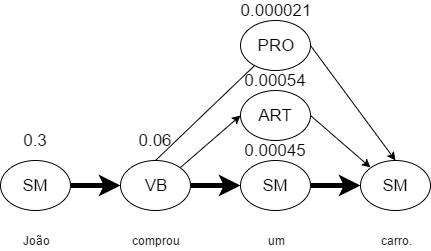
\includegraphics[height=180px]{imagens/markov2.png}
\caption{Caminhos definidos para a classificação pelo Algoritmo de Viterbi}
\label{fig:markov2}
\end{figure}


% Uma maneira de diferenciarmos os dois métodos é através do problema de
% ambiguidade. Por exemplo, nas frases:
%
% ``João entrou no carro conversível de óculos novos.''. E ``João entrou no carro
% conversível de farol apagado.''.
%
% Em ambas as frases, após a preposição ``de'' segue um substantivo masculino.
% Porém, cada uma das frases se refere a um substantivo diferente. A
% primeira se refere ao João, visto que não existe sentido em um carro ter óculos.
% Já a segunda se refere ao próprio carro, visto que não existe sentido em João
% ter faróis.
%
% O método simbólico para resolver esse problema faz a criação de novas regras se
% baseadas no conhecimento humano para a solução de qual o significado da frase.
% Já o método estatístico, irá verificar qual a probabilidade de cada significado
% para cada frase através de análises similares decidindo através de metódos
% estatísticos qual o significado correto para cada frase
% \cite{jacksonmoulinier2007}.

